\documentclass[12pt, class=report, crop=false]{standalone}
\usepackage{msc_thesis}
\usepackage{wrapfig}

% !TeX spellcheck = en-GB
% !TEX bib = reference.bib
% chktex-file 21 # This command might not be intended.

\begin{document}

\chapter{Particle in Cell Method}%
\label{chap:pic}

As we outlined in Chapter~\ref{chap:classical-electrodynamics}, the interaction
of some charged particles with an electromagnetic field can be viewed as the
action of the sources on the fields and the action of the fields on the sources.

In the same manner, simulating the interaction self-consistently requires a
\emph{field solver} that computes the structure of the fields considering
the sources and a \emph{particle pusher} that solves the (relativistic)
equations of motion for the particles.
In the particle in cell method, a finite-difference time-domain (FDTD) method
is used for solving Maxwell's equations and a modified leapfrog method is used
for the particle pusher as presented in~\cite{arber_contemporaryparticleincell_2015}.

\section{Numerical Methods Introduction}

The numerical methods mentioned above are based on the idea of discretizing the
derivative operator. There are multiple ways of discretizing this operator,
but all of them can be derived from the Taylor series expansion.
\[
  f(x_0+h) = f(x_0) + \frac{f'(x_0)}{1!}h + \frac{f''(x_0)}{2!}h^2 + \dotsb + \frac{f^{(n)}(x_0)}{n!}h^n + \dots
\]

The main discretizations options are the forward, backward and central differences.
For the forward discretization we consider
\[
  f(x_0+h) = f(x_0) + \frac{f'(x_0)}{1!}h + \frac{f''(x_0)}{2!}h^2 + \dotsb
\]
and we rearrange the terms in the following way
\[
  \frac{f(x_0+h) - f(x_0)}{h} = f'(x_0) + \frac{f''(x_0)}{2}h + \dotsb
\]
and thus, when \(h \to 0\), the derivative in first order is given by
\[
  f'(x_0) = \frac{f(x_0+h) - f(x_0)}{h} + \order{h}\,.
\]

The local truncation error is given by the error of the approximation in one time
step. The forward and backward discretizations are both of order one. The
central discretization is second order accurate and can be derived as follows.

We first begin with the forward and backward discretizations for half of a
timestep:
\begin{align*}
  f(x_0+\frac{h}{2}) &= f(x_0) + f'(x_0)\frac{h}{2} + \frac{f''(x_0)}{2}\frac{h^2}{4}
    + \frac{f^{(3)}(x_0)}{3!}\frac{h^3}{8} + \dotsb \\
  f(x_0-\frac{h}{2}) &= f(x_0) - f'(x_0)\frac{h}{2} + \frac{f''(x_0)}{2}\frac{h^2}{4}
    - \frac{f^{(3)}(x_0)}{3!}\frac{h^3}{8} + \dotsb \,.
\end{align*}

Then we take the difference and obtain
\[
  f(x_0+\frac{h}{2}) - f(x_0-\frac{h}{2}) = f'(x_0)h
    + 2\frac{f^{(3)}(x_0)}{3!}\frac{h^3}{8} + \dotsb
\]
and we can see that indeed the central difference is second order accurate
\[
  f'(x_0) = \frac{f(x_0+\frac{h}{2}) - f(x_0-\frac{h}{2})}{h} + \order{h^2}\,.
\]

As an application of the methods discussed above, we will now derive the so called
leapfrog method for solving second order differential equations
following~\textcite[Chapter~4]{hockney_computersimulation_1988}. More concretely,
we will take a look at solving the equations of motion for a particle. As a first
step, the equations of motion can be written as a system of first order differential
equations
\begin{align*}
  \dv{\vb{x}}{t} &= \vb{v} \\
  m \dv{\vb{v}}{t} &= \vb{F}\,,
\end{align*}
where \(\vb{F}\) is the total force on the particle. Replacing the derivatives
with their finite difference approximations, we obtain
\begin{subequations}
  \begin{align}
    \label{eq:leapfrog}
    \frac{\vb{x}_{n+1} - \vb{x}_n}{\Delta t} = \vb{v}_{n+1/2} \\
    m \frac{\vb{v}_{n+1/2} - \vb{v}_{n-1/2}}{\Delta t} = \vb{F}(\vb{x}_n)\,.
  \end{align}
\end{subequations}
Replacing the velocity, we obtain
\begin{equation*}
  % \label{eq:leapfrog-no-v}
  \frac{\vb{x}_{n+1}-2\vb{x}_n+\vb{x}_{n-1}}{\Delta t^2} = \frac{\vb{F}(\vb{x}_n)}{m}\,.
\end{equation*}

\subsection{Accuracy}

The accuracy of an integration method is given by difference between the true
solution and the approximate solution at a given timestep, that is the local
error. There are two types of local errors: truncation errors and roundoff errors.
Truncation errors are given by the approximations employed in the numerical method.
On the other hand, roundoff errors are consequence of implementing the numerical
method on a computer with finite precision. In general, for low order methods,
the truncation errors are significantly bigger than roundoff errors, and thus
we can consider that the accuracy is given only by truncation error.

In order to better illustrate the concept of truncation errors, we will exemplify
its computation for the leapfrog method. Let us consider the local truncation
error at the timestep \(n\), \(\delta^n\) and \(\vb{X}\) the true solution
\[
  \frac{\vb{X}_{n+1}-2\vb{X}_n+\vb{X}_{n-1}}{\Delta t^2} = \frac{\vb{F}(\vb{X}_n)}{m} + \delta^n\,.
\]

If we expand \(\vb{X}_{n+1}\) and \(\vb{X}_{n-1}\) in Taylor series around \(\vb{X}_n\)
\begin{align*}
  \vb{X}_{n+1} &= \vb{X}_n + \dv{\vb{X}_n}{t}\Delta t + \frac{1}{2} \dv[2]{\vb{X}_n}{t} - \dotsb \\
  \vb{X}_{n-1} &= \vb{X}_n - \dv{\vb{X}_n}{t}\Delta t + \frac{1}{2} \dv[2]{\vb{X}_n}{t} - \dotsb\,,
\end{align*}
we obtain
\[
  \dv[2]{\vb{X}_n}{t} + \frac{\Delta t^2}{12} \dv[4]{\vb{X}}{t} + \order{\Delta t^5}
  = \frac{\vb{F}(\vb{X}_n)}{m} + \delta^n\,,
\]
and thus
\[
  \delta^n \sim \order{\Delta t^2}
\]
which shows that the leapfrog algorithm is of order 2.

\subsection{Stability}

A numerical method is considered asymptotically stable if the solution obtained
for a linear problem is asymptotically bounded.
As in the previous case we will show an example for the leapfrog method,
following the ideas exposed in~\cite{butcher_numericalmethods_2016}
and in~\textcite[Section 2.6]{leimkuhler_simulatinghamiltonian_2004}.

A linear problem can be written as
\[
\dv{t} \vb{z} = A \vb{z}\,,
\]
where we used the following notation to denote the dynamical state of the system
\[
\vb{z} =
\begin{pmatrix}
  \vb{q} \\
  \vb{p}
\end{pmatrix}\,.
\]

The solution can be written as
\begin{equation*}
  % \label{eq:linear-problem-solution}
  \vb{z}(t) = R(t) \vb{z}_0\,,
\end{equation*}
where \(R(t)\) is a matrix which can give the solution at any time by evolving
the initial conditions.

The discrete version of the problem is given by
\begin{equation}
  \label{eq:discrete-linear-problem}
  \vb{z}_{n+1} = \hat{R}(\Delta t) \vb{z}_n\,,
\end{equation}
where \(\hat{R}(\Delta t)\) is called the propagation matrix.
With this considerations, asymptotic stability can be expressed as a function
of the eigenvalues of \(\hat{R}(\Delta t)\), since the solution is obtained
with powers of \(\hat{R}\) from the initial conditions
\begin{equation*}
  % \label{eq:discrete-linear-solution}
  \vb{z}_n = {[\hat{R}]}^n \vb{z}_0\,.
\end{equation*}

More concretely, a method is asymptotically stable if the eigenvalues of
\(\hat{R}\) are inside the unit disk in the complex plane and simple (not repeated)
if on the unit circle~\autocite[28]{leimkuhler_simulatinghamiltonian_2004}.

One of the most studied linear problems is the harmonic oscillator and we can use
it as our model linear problem
\[
\mathcal{H} = \frac{\vb{p}^2}{2m} + \frac{\omega^2 \vb{q}^2}{2}\,.
\]

The equations of motion are given by the corresponding Hamilton equations
\begin{align*}
  \dot{q}_i &= \pdv{\mathcal{H}}{p_i} = \frac{p_i}{m} \\
  \dot{p}_i &= -\pdv{\mathcal{H}}{q_i} = -\omega^2 q_i\,.
\end{align*}

Taking \(m=1\) and writing the above equations in matrix form yields
\[
\dot{\vb{z}} =
\begin{pmatrix}
  p \\
  -\omega^2 q
\end{pmatrix} =
\begin{pmatrix}
  0 & 1 \\
  -\omega^2 & 0
\end{pmatrix}
\begin{pmatrix}
  \vb{q} \\
  \vb{p}
\end{pmatrix}
\]
and thus we obtain
\[
\dot{\vb{z}} = A \vb{z},
\]
with
\[
A =
\begin{pmatrix}
  0 & 1 \\
  -\omega^2 & 0
\end{pmatrix}\,.
\]

The solution is given by
\[
\vb{z}(t) = R(t) \vb{z}_0,
\]
with
\[
R(t) =
\begin{pmatrix}
  \cos(\omega t) & \frac{1}{\omega} \sin(\omega t) \\
  -\omega \sin(\omega t) & \cos(\omega t)
\end{pmatrix}\,.
\]

In order to analyze the stability of the leapfrog algorithm, it is convenient to
express the equations in a different form, also called the Störmer–Verlet method
\begin{align*}
  \vb{q}_{n+1} &= \vb{q}_n + \Delta t \vb{v}_{n+1/2} \\
  M \vb{v}_{n+1/2} &= M \vb{v}_n - \frac{\Delta t}{2} \grad{V(\vb{q}_n)} \\
  M \vb{v}_{n+1} &= M \vb{v}_{n+1/2} - \frac{\Delta t}{2} \grad{V(\vb{q}_{n+1})}\,.
\end{align*}

In our particular case, the gradient of the potential is given by
\(\omega^2 q\) and the above reduces to
\begin{align*}
  \vb{q}_{n+1} &= \vb{q}_n + \Delta t (\vb{v}_n - \frac{\Delta t}{2} \omega^2 \vb{q}^n) =
  \vb{q}_n \left(1 - \frac{\Delta t^2 \omega^2}{2}\right) + \vb{v}_n \Delta t \\
  \vb{p}_{n+1} &= \vb{p}_n - \frac{\Delta t^2}{2} \omega^2 \vb{q}_n
  -\frac{\Delta t^2}{2} \omega^2 \vb{q}_{n+1} =
  \vb{p}_n - \frac{\Delta t^2}{2} \omega^2 \vb{q}_n
  -\frac{\Delta t}{2}\omega^2 \left(\vb{q}_n+\vb{v}_n-\frac{\Delta t}{2}\omega^2 \vb{q}_n\right)\,,
\end{align*}
or
\[
\begin{pmatrix}
  \vb{q}_{n+1} \\
  \vb{p}_{n+1}
\end{pmatrix} =
\begin{pmatrix}
  1 - \frac{\Delta t^2 \omega^2}{2} & \Delta t \\
  -\Delta t \omega^2 \left(1 - \frac{\Delta t^2 \omega^2}{4}\right) &
  1 - \frac{\Delta t^2 \omega^2}{2}
\end{pmatrix}
\begin{pmatrix}
  \vb{q}_n \\
  \vb{p}_n
\end{pmatrix}\,.
\]

Comparing with \cref{eq:discrete-linear-problem} we obtain
\[
\hat{R}(\Delta t) =
\begin{pmatrix}
  1 - \frac{\Delta t^2 \omega^2}{2} & \Delta t \\
  -\Delta t \omega^2 \left(1 - \frac{\Delta t^2 \omega^2}{4}\right) &
  1 - \frac{\Delta t^2 \omega^2}{2}
\end{pmatrix}\,.
\]

The eigenvalues of \(\hat{R}\) are given by the solution of
\(
\det(\hat{R} - \lambda I) = 0
\), or more explicitly
\[
\vmqty{
1 - \frac{\Delta t^2 \omega^2}{2} & \Delta t \\
-\Delta t \omega^2 \left(1 - \frac{\Delta t^2 \omega^2}{4}\right) &
1 - \frac{\Delta t^2 \omega^2}{2}
} = 0\,.
\]

This reduces to
\[
{\left(1-\frac{\Delta t^{2} \omega^2}{2}-\lambda\right)}^{2}+
\frac{\Delta t^{2} \omega^2}{2}\left(2-\frac{\Delta t^2 \omega^2}{2}\right) = 0\,.
\]
Using the notation \(\frac{\Delta t^{2} w^{2}}{2}\equiv\mu^{2}\),
we obtain
\[
{\left(1-\mu^{2}-\lambda\right)}^2+\mu^{2}\left(2-\mu^{2}\right)=0\,,
\]
which can be further expanded to
\[
\lambda^{2}+{\left(1-\mu^{2}\right)}^{2}-2\left(1-\mu^{2}\right) \lambda+\mu^{2}\left(2-\mu^{2}\right)=0\,,
\]
yielding the solutions
\begin{align*}
  \lambda_{1,2} &= \frac{1}{2} \left\{2(1-\mu^2) \pm
  \sqrt{4{(1-\mu^2)}^2 - 4\left[{(1-\mu^2)}^2 + \mu^2 (2-\mu^2)\right]}\right\} \\
  &= 1-\mu^2 \pm \sqrt{\mu^2(\mu^2-2)}\,.
\end{align*}

We notice that for \(\mu^2 < 2\) the solutions are complex and
\begin{align*}
  |\lambda_{1,2}|^2 &= (1-\mu^2) + \mu^2 (\mu^2-2) \\
  &= 1+\mu^4-2\mu^2+\mu^4-2\mu^2 \\
  &= 1+\mu^4-4\mu^2\,.
\end{align*}

The method will be stable for \(|\lambda|^2 < 1\), or
\[
\mu^2 (\mu^2 - 4) < 0 \implies \mu < 2, \text{for } \mu \ne 0\,.
\]

For \(\mu^2 > 2\) the eigenvalues are real and with modulus greater than 1.
Thus the stability condition for the Störmer–Verlet method is given by \(\mu < 2\),
or
\[
\Delta t^2 \omega^2 < 4\,,
\]
indicating a sampling of at least \(\pi\) points per period, or a step size
\(\Delta t < 2/\omega\).

In the context of ordinary differential equations, a stability region of the method
is usually defined via a stability function \(R(z)\) in the complex
plane~\autocite[81]{butcher_numericalmethods_2016}. Such approach cannot be used
in this case since the stability function is defined for a singe ordinary
differential equation, but in the case of Hamiltonian dynamics we always have
\(2n\) ordinary differential equations, with \(n>1\).

\section{The particle pusher}

Having (briefly) developed some general aspects of the theory of numerical methods
for solving differential equations, we now continue with the more concrete case
of numerically solving the equations of motion for a charged particle.
In the non-relativistic case, the (continuous) equations of motion have the
following form
\begin{align*}
  \dv{\vb{x}}{t} &= \vb{v} \\
  \dv{\vb{v}}{t} &= \frac{q}{m} \left(\vb{E} + \vb{v}\cp\vb{B}\right)\,.
\end{align*}

Since the above equations are symmetric with respect to time reversal, it is
desired that we obtain a discretization which is also time-reversible.
\Textcite{buneman_timereversibledifference_1967} explained that we can
use centered differences for this task and in the particular case of the
Lorentz force we can average the velocity in order to represent the
\(\vb{v} \cp \vb{B}\) product symmetrically. Thus we obtain
\begin{subequations}
  \begin{align}
    \label{eq:lorentz-discrete-x}
    \frac{\vb{x}_{n+1}-\vb{x}_n}{\Delta t} &= \vb{v}_{n+1} \\
    \label{eq:lorentz-discrete-v}
    \frac{\vb{v}_{n+1/2}-\vb{v}_{n-1/2}}{\Delta t} &= \frac{q}{m}
      \left(\vb{E}(\vb{x}_n) + \frac{\vb{v}_{n+1/2}+\vb{v}_{n-1/2}}{2} \cp \vb{B}(\vb{x}_n)\right)\,.
  \end{align}
\end{subequations}

As explained in~\textcite[Chapter 4--3]{birdsall_plasmaphysics_2005}, there are
several methods for solving the above equations, implying a
partial~\autocite{buneman_timereversibledifference_1967} or
complete~\autocite{boris_relativisticplasma_1970} separation of the electric
and magnetic force contributions. In the following we will detail the second
method, which is also called the Boris push.

Let us introduce the following notation
\begin{align*}
  \vb{v}^- &= \vb{v}_{n-1/2} - \frac{q \vb{E}}{m} \frac{\Delta t}{2} \\
  \vb{v}^+ &= \vb{v}_{n+1/2} + \frac{q \vb{E}}{m} \frac{\Delta t}{2}\,,
\end{align*}
such that
\[
\frac{\vb{v}^+ - \vb{v}^-}{\Delta t} = \frac{\vb{v}_{n+1/2} - \vb{v}_{n-1/2}}{\Delta t}
+ \frac{q \vb{E}}{m}\,.
\]

Substituting in \cref{eq:lorentz-discrete-v} we obtain
\begin{equation}
  \label{eq:vp-vm-rotation}
  \frac{\vb{v}^+ - \vb{v}^-}{\Delta t} = \frac{q}{2m} (\vb{v}^+ + \vb{v}^-) \cp \vb{B}\,,
\end{equation}
which can be seen as a rotation. Indeed, if we take the scalar product with
\((\vb{v}^+ + \vb{v}^-)\), we get
\[
(\vb{v}^+ + \vb{v}^-) \vdot \frac{\vb{v}^+ - \vb{v}^-}{\Delta t} =
\frac{q}{2m} \underbrace{(\vb{v}^+ + \vb{v}^-) \vdot (\vb{v}^+ + \vb{v}^-) \cp \vb{B}}_{0}
\]
or
\[
|\vb{v}^+|^2 - |\vb{v}^-|^2 = 0\,,
\]
implying that \(|\vb{v}^+| = |\vb{v}^-|\).

If we decompose the \(\vb{v}^-\) into its parallel and perpendicular components
with respect to \(\vb{B}\), we can reduce the rotation of \(\vb{v}^-\) to
the rotation of its perpendicular component \(\vb{v}^-_\perp\).

\begin{wrapfigure}[10]{r}{0.4\textwidth}
  \centering
  \subimport{../figures/}{Boris-rotation-angle}%
  \caption{Boris rotation angle}\label{fig:Boris-rotation-angle}%
\end{wrapfigure}

The angle of rotation between \(\vb{v}^-_\perp\) and \(\vb{v}^-_\perp\),
denoted with \(\theta\) in \cref{fig:Boris-rotation-angle},
can be expressed as
\[
\tan{\frac{\theta}{2}} = \frac{|\vb{v}^+_\perp - \vb{v}^-_\perp|}{|\vb{v}^+_\perp + \vb{v}^-_\perp|}\,.
\]

Rewriting \cref{eq:vp-vm-rotation} we obtain
\[
\vb{v}^+ - \vb{v}^- = \frac{q \Delta t}{2m} (\vb{v}^+ + \vb{v}^-) \cp \vb{B}
\]
and if we substitute \(\vb{v}^\pm = \vb{v}^\pm_\perp + \vb{v}^\pm_\parallel\)
\[
\vb{v}^+_\perp - \vb{v}^-_\perp = \frac{q \Delta t}{2m} (\vb{v}^+_\perp + \vb{v}^-_\perp) \cp \vb{B}\,.
\]

Furthermore, since all the vectors above have the same direction by construction,
we can factor out the versors and obtain
\[
\frac{|\vb{v}^+_\perp - \vb{v}^-_\perp|}{|\vb{v}^+_\perp + \vb{v}^-_\perp|} =
\frac{q |\vb{B}|}{m} \frac{\Delta t}{2}
\]
and thus
\begin{equation}
  \label{eq:Boris-rotation-angle}
  \tan{\frac{\theta}{2}} = \frac{q B}{m} \frac{\Delta t}{2}\,.
\end{equation}

Since for the rotation described above only the components perpendicular to
the direction of \(\vb{B}\) matter, we can simplify the notation and use
\(\vb{v}_\pm\) instead of \(\vb{v}^\pm_\perp\).
We will now introduce an additional vector \(\vb{v}'\) given by the addition
between \(\vb{v}_-\) and another vector, such that \(\vb{v}'\) is perpendicular
to \(\vb{v}_+ - \vb{v}_-\).

It is convenient to write \(\vb{v}'\) as \(\vb{v}' = \vb{v}_- + \vb{v}_- \cp \vb{t}\).
In the right triangle formed by \(\vb{v}'\) with \(\vb{v}_-\)
and \(\vb{v}_- \cp \vb{t}\) as seen in \cref{fig:Boris-rotation-3D},
we have
\[
\tan{\frac{\theta}{2}} = \frac{|\vb{v}_- \cp \vb{t}|}{|\vb{v}_-|} = |\vb{t}|
\]
and thus by using \cref{eq:Boris-rotation-angle} \(\vb{t}\) is given by
\[
\vb{t} = \frac{q \vb{B}}{m} \frac{\Delta t}{2}\,.
\]

\begin{figure}[H]
  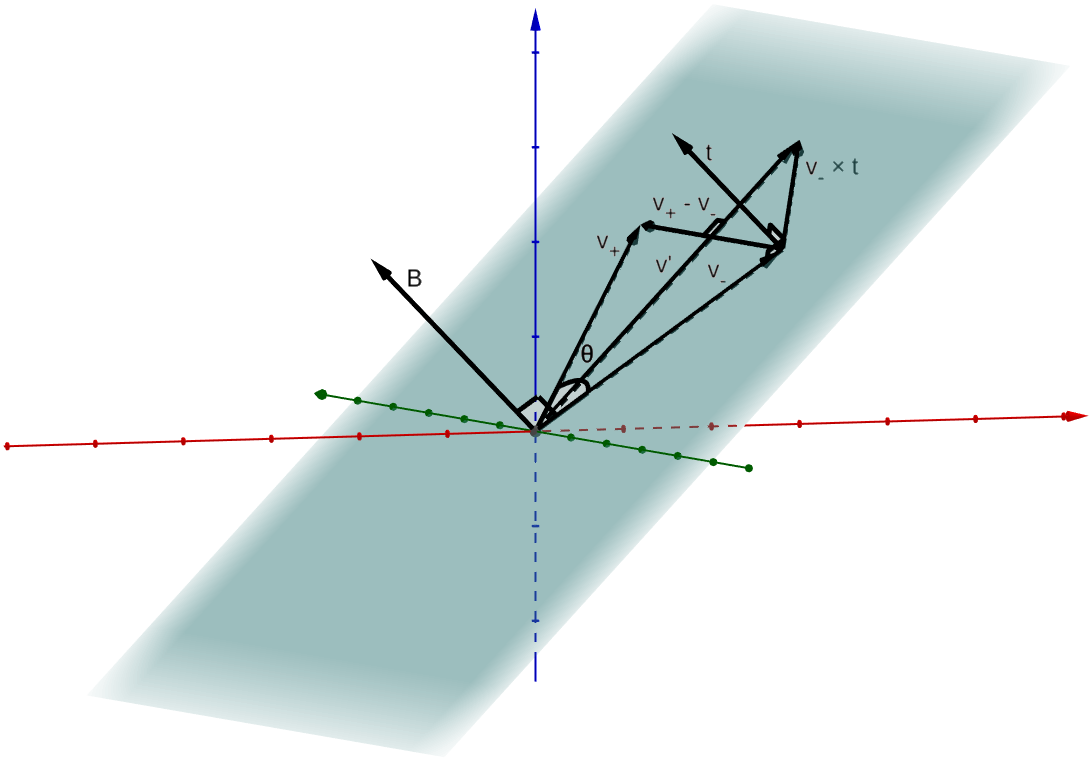
\includegraphics[width=\textwidth]{Boris-rotation-3D}
  \caption{Boris rotation construction in 3D}%
  \label{fig:Boris-rotation-3D}%
\end{figure}

As can be seen in \cref{fig:Boris-rotation-3D},
\(\vb{v}_+ - \vb{v}_- \parallel \vb{v}' \cp \vb{B}\). This encourages
the following notation: \(\vb{v}_+ - \vb{v}_- \equiv \vb{v}' \cp \vb{s}\),
where \(\vb{s}\) can be determined by the condition that
\(|\vb{v}_+|^2 = |\vb{v}_-|^2\). Thus, expanding \(\vb{v}' \cp \vb{s}\) gives
\[
\vb{v}' \cp \vb{s} = (\vb{v}_- + \vb{v}_- \cp \vb{t}) \cp \vb{s} =
\vb{v}_- \cp \vb{s} + \vb{t} \underbrace{(\vb{v}_- \vdot \vb{s})}_0 - \vb{v}_- (\vb{t} \vdot \vb{s})
\]

\begin{wrapfigure}[15]{r}{0.4\textwidth}
  \centering
  \subimport{../figures/}{Boris-rotation-construction}%
  \caption{The velocities projected in the plane perpendicular to \(\vb{B}\)}\label{fig:Boris-rotation-construction}%
\end{wrapfigure}

and if we consider the definition for \(\vb{s}\)
\[
\vb{v}_+ = \vb{v}_- + \vb{v}' \cp \vb{s} =
\vb{v}_- + \vb{v}_- \cp \vb{s} - \vb{v}_- (\vb{t} \vdot \vb{s})\,.
\]
Taking the scalar product with \(\vb{v}_-\) gives
\[
\vb{v}_+ \vdot \vb{v}_- = |\vb{v}_-|^2 - |\vb{v}_-|^2 (\vb{t} \vdot \vb{s})
\]
or
\[
|\vb{v}_-|^2 \cos{\theta} = |\vb{v}_-|^2 (1 - \vb{t} \vdot \vb{s})\,.
\]

Using the trigonometry identity
\[
\cos{\theta} = \frac{1-\tan^2{\frac{\theta}{2}}}{1+\tan^2{\frac{\theta}{2}}}\,,
\]
we obtain
\[
\vb{t} \vdot \vb{s} = 1 - \frac{1-\tan^2{\frac{\theta}{2}}}{1+\tan^2{\frac{\theta}{2}}}\,,
\]
which is equivalent to
\[
\vb{t} \vdot \vb{s} = \frac{2 t^2}{1+t^2}
\]
and thus we obtain that
\[
\vb{s} = \frac{2 \vb{t}}{1+t^2}\,.
\]

As a summary, the Boris push algorithm solves \cref{eq:lorentz-discrete-v} with the following steps:
\begin{enumerate}
  \item \(\vb{v}^- = \vb{v}_{n-1/2} + \frac{q \vb{E}}{m} \frac{\Delta t}{2}\)
  \item rotate \(\vb{v}^-\) to obtain \(\vb{v}^+\) using
  \begin{enumerate}
    \item \(\vb{v}' = \vb{v}^- + \vb{v}^- \cp \vb{t}\), where \(\vb{t} = \frac{q \vb{B}}{m} \frac{\Delta t}{2}\)
    \item \(\vb{v}^+ = \vb{v}^- + \vb{v}' \cp \vb{s}\), where \(\vb{s} = \frac{2 \vb{t}}{1+t^2}\)
  \end{enumerate}
  \item \(\vb{v}_{n+1/2} = \vb{v}^+ + \frac{q \vb{E}}{m} \frac{\Delta t}{2}\)
\end{enumerate}

\subsection{Conservation properties}

When solving (continuous) differential equations with (discrete) numerical methods,
an important aspect is that we want the algorithm to be as close as possible to
the original continuous system in terms of symmetries and conserved
quantities~\autocite{stuart_dynamicalsystems_1996}.

In what follows we will look at the conservation properties of the Boris push
and show why are they important for simulating the dynamics of charged particles
following the ideas presented in~\textcite{qin_whyboris_2013}.

Mathematically speaking, a Hamiltonian system is given by the phase space (an
even dimensional manifold\footnote{A manifold is a topological space that is locally Euclidean.}),
a symplectic structure on it and the Hamiltonian
function~\autocite[160]{arnold_mathematicalmethods_1989}.
In order to explain what the symplectic structure is, we will start with a short
discussion about 2-forms~\autocite[164]{arnold_mathematicalmethods_1989}.

\begin{definition*}
  An exterior form of degree 2 (or a 2-form) is a function of pairs of vectors
  \(\omega^2: \mathbb{R}^n \cp \mathbb{R}^n\), which is bilinear and skew symmetric:
  \begin{align*}
  \omega^2(\lambda_1 \vb*{\xi}_1 + \lambda_2 \vb*{\xi}_2, \vb*{\xi}_3) &=
  \lambda_1 \omega^2(\vb*{\xi}_1, \vb*{\xi}_3) + \lambda_2 \omega^2(\vb*{\xi}_2, \vb*{\xi}_3) \\
  \omega^2(\vb*{\xi}_1,\vb*{\xi}_2) &= -\omega^2(\vb*{\xi}_2, \vb*{\xi}_1)\,,
  \end{align*}
  \(\forall \lambda_{1,2} \in \mathbb{R}, \vb*{\xi}_{1,2,3} \in \mathbb{R}^n\).
\end{definition*}

As an example of a 2-form in \(n=2\) dimensions is given by the \emph{oriented area} spanned by 2 vectors
in the (oriented) euclidean plane \(\mathbb{R}^2\).
Let us consider
\[
\vb*{\xi} = \mqty(\xi_1 \\ \xi_2), \qquad
\vb*{\eta} = \mqty(\eta_1 \\ \eta_2)\,,
\]
then the oriented are determined by the two vectors is given by
the determinant~\autocite{golomb_proofwords_1985}
\[
S(\vb*{\xi},\vb*{\eta}) = \det\mqty(\xi_1 & \eta_1 \\ \xi_2 & \eta_2)
= \xi_1 \eta_2 - \xi_2 \eta_1\,.
\]

Let us consider an \(2d\)-dimensional phase space with the coordinates \(q_i,p_i\) as presented in~\textcite[183]{leimkuhler_simulatinghamiltonian_2004}.

\begin{definition}
  A linear map \(A: \mathbb{R}^{2d} \to \mathbb{R}^{2d}\) is called
  \emph{symplectic} if there exists a 2-form \(\omega\)
  such that
  \[
  \omega(A\vb*{\xi}, A\vb*{\eta}) = \omega(\vb*{\xi},\vb*{\eta})\,,\
  \forall \vb*{\xi}, \vb*{\eta} \in \mathbb{R}^{2d}\,.
  \]
\end{definition}

We can also express the above in matrix notation
\[
A^T J^{-1} A = J^{-1},\qquad \text{where} \ J = \mqty(0 & I \\ -I & 0)\,,
\]
with \(I\) the identity matrix in \(d\) dimensions.

A useful example that illustrates the concept is given in the case of \(d=1\),
where symplecticity implies area conservation under the given
linear transformation. In the more general \(d>1\) case, it would imply the conservation of the sum
of the respective projected areas.

As we have seen from the beginning of this chapter, differentiable
functions are often approximated using linear maps. This provides
the motivation for extending the above definition to the non-linear case.

\begin{definition}%
  \label{def:symplecticity-nonlinear}
  A differentiable map \(g:U \to \mathbb{R}^{2d}\), with \(U \subset \mathbb{R}^{2d}\) an open set, is called
  \emph{symplectic} if its corresponding Jacobian matrix \(g'(\vb{p},\vb{q})\) is everywhere symplectic, i.e.
  \[
  \omega(g'(\vb{p},\vb{q})\vb*{\xi}, g'(\vb{p},\vb{q})\vb*{\eta}) =
  \omega(\vb*{\xi},\vb*{\eta})
  \]
  or in matrix notation \({g'(\vb{p},\vb{q})}^T J^{-1} g'(\vb{p},\vb{q}) = J^{-1}\).
\end{definition}

Having defined symplecticity, we will now try to check if the Boris
push algorithm is symplectic. For this task we begin with rewriting
\cref{eq:lorentz-discrete-v} in a more convenient form
\[
\vb{v}_{n+1/2} - \frac{q \Delta t}{2m} \vb{v}_{n+1/2} \cp \vb{B}_n =
\vb{v}_{n-1/2} + \frac{q \Delta t}{2m} \vb{v}_{n-1/2} \cp \vb{B}_n
+ \frac{q \Delta t}{m} \vb{E}_n\,,
\]
where \(\vb{B}_n \equiv \vb{B}(\vb{x}_n)\) and
\(\vb{E}_n \equiv \vb{E}(\vb{x}_n)\).

In order to manipulate the above more easily, it is useful to introduce some fundamental group theory notions~\autocite[118]{hairer_geometricnumerical_2006} and the hat map~\autocite[289]{marsden_introductionmechanics_1999}.

\begin{definition}
  A \emph{Lie group} \(G\) is a group that is also a differentiable
  manifold and for which the product is given by the differentiable
  mapping \(G \cp G \to G\).
\end{definition}

The tangent space \(\mathfrak{g} = T_I G\) at the identity \(I\)
of a matrix Lie group \(G\) is closed under forming commutators
of its elements and defines the \emph{Lie algebra} of \(G\).

\begin{definition}
  The \emph{hat map} \(\hat{}: \mathbb{R}^3 \to \mathfrak{so}(3)\) is a
  vector space isomorphism that identifies the Lie algebra \(\mathfrak{so}(3)\)
  of \(SO(3)\) with \(\mathbb{R}^3\). If we consider
  \(\vb{v} = (v_1,v_2,v_3) \in \mathbb{R}^3\), then the hat map
  is given by
  \[
    \hat{\vb{v}} =
    \begin{pmatrix}
      \phantom{-}0\phantom{_1} & -v_3           & \phantom{-}v_2 \\
      \phantom{-}v_3 & \phantom{-}0\phantom{_1} &           -v_1 \\
            -v_2     & \phantom{-}v_1 &\phantom{-}0\phantom{_1}
    \end{pmatrix}\,.
  \]
\end{definition}

We can observe that
\[
\hat{\vb{v}} \vb{w} = \vb{v} \cp \vb{w}
\]
characterizes the isomorphism. Comparing
\[
\hat{\vb{v}} \vb{w} =
\begin{pmatrix}
  \phantom{-}0\phantom{_1} & -v_3           & \phantom{-}v_2 \\
  \phantom{-}v_3 & \phantom{-}0\phantom{_1} &           -v_1 \\
        -v_2     & \phantom{-}v_1 &\phantom{-}0\phantom{_1}
\end{pmatrix}
\begin{pmatrix}
  w_1 \\
  w_2 \\
  w_3
\end{pmatrix}
=
\begin{pmatrix}
            -v_3 w_2 + v_2 w_3 \\
  \phantom{-}v_3 w_1 - v_1 w_3 \\
            -v_2 w_1 + v_1 w_2
\end{pmatrix}
\]
with
\[
(\vb{v} \cp \vb{w}) = \vb{e}_i \epsilon_{ijk} v_j w_k =
\vb{e}_1 (v_2 w_3 - v_3 w_2) + \vb{e}_2 (v_3 w_1 - v_1 w_3) +
\vb{e}_3 (v_1 w_2 - v_2 w_1)
\]
we can see that this is indeed true.

Thus, if we consider \(\mathbb{R}^3\) together with the cross product,
the hat map \(\hat{}\)\ becomes a Lie algebra isomorphism and we
can identify \(\mathfrak{so}(3)\) with \(\mathbb{R}^3\) having the
cross product as Lie bracket\footnote{A bilinear, skew symmetric operation \(\mathfrak{g}\cp\mathfrak{g}\to\mathfrak{g}\) that
satisfies the Jacobi identity.}.

We can now resume rewriting \cref{eq:lorentz-discrete-v} and we obtain
\begin{equation}
\label{eq:lorentz-v-hat-map}
\left(I - \hat{\Omega}_{n}\right)
\begin{pmatrix}
  v_{n+1/2}^1 \\
  v_{n+1/2}^2 \\
  v_{n+1/2}^3
\end{pmatrix}
=
\left(I + \hat{\Omega}_{n}\right)
\begin{pmatrix}
  v_{n-1/2}^1 \\
  v_{n-1/2}^2 \\
  v_{n-1/2}^3
\end{pmatrix}
+ \frac{q \Delta t}{m}
\begin{pmatrix}
  E_n^1 \\
  E_n^2 \\
  E_n^3
\end{pmatrix}\,,
\end{equation}
where
\[
\hat{\Omega}_n =
\frac{q \Delta t}{2m}
\begin{pmatrix}
  \phantom{-}0\phantom{_1} & -B^3_n & \phantom{-}B^2_n \\
  \phantom{-}B^3_n & \phantom{-}0\phantom{_1} & -B^1_n \\
  -B^2_n & \phantom{-}B^1_n & \phantom{-}0\phantom{_1}
\end{pmatrix}\,.
\]

Multiplying on the left of \cref{eq:lorentz-v-hat-map} with
\(\left(I - \hat{\Omega}_{n}\right)\) yields
\[
\begin{pmatrix}
  v_{n+1/2}^1 \\
  v_{n+1/2}^2 \\
  v_{n+1/2}^3
\end{pmatrix}
=
{\left(I - \hat{\Omega}_{n}\right)}^{-1} \left(I + \hat{\Omega}_{n}\right)
\begin{pmatrix}
  v_{n-1/2}^1 \\
  v_{n-1/2}^2 \\
  v_{n-1/2}^3
\end{pmatrix}
+ \frac{q \Delta t}{m} {\left(I - \hat{\Omega}_{n}\right)}^{-1}
\begin{pmatrix}
  E_n^1 \\
  E_n^2 \\
  E_n^3
\end{pmatrix}\,.
\]

In order to further simplify the notation, we can use the following notation:
\(\vb{x}_n \equiv \vb{x}_k\) and \(\vb{v}_{n-1/2} \equiv \vb{v}_k\)
and use the Cayley transform
for the first term on the right hand side.
For a quadratic Lie group\footnote{Lie groups of the form
\(G = \set{Y ; Y^T P Y = P}\), where \(P\) is a constant
matrix.}, the \emph{Cayley transform}
\[
\cay{\Omega} = {(I-\Omega)}^{-1} (I+\Omega)
\]
maps elements of \(\mathfrak{g}\) into \(G\)~\autocite[128]{hairer_geometricnumerical_2006}.

In our particular case
\[
{\left(I - \hat{\Omega}_{n}\right)}^{-1} \left(I + \hat{\Omega}_{n}\right) = \cay{\hat{\Omega}_{n}} \equiv R
\]
and we obtain
\[
\vb{v}_{k+1} = R \vb{v}_k + \frac{q \Delta t}{m} {\left(I - \hat{\Omega}_{n}\right)}^{-1} \vb{E}_k\,.
\]

Thus \cref{eq:lorentz-discrete-x,eq:lorentz-discrete-v} form a
one step map \(\Psi_B\) which maps \(\vb{z}_k \equiv (\vb{x}_k, \vb{v}_k)\)
to \(\vb{z}_{k+1} \equiv (\vb{x}_{k+1}, \vb{v}_{k+1})\)
\begin{equation*}
  \Psi_B: \left\{
  \begin{aligned}
    \vb{x}_{k+1} &= \vb{x}_k + R \Delta t\vb{v}_k + \frac{q \Delta t}{m} {\left(I - \hat{\Omega}_{n}\right)}^{-1} \vb{E}_k \\
    \vb{v}_{k+1} &= R \vb{v}_k + \frac{q \Delta t^2}{m} {\left(I - \hat{\Omega}_{n}\right)}^{-1} \vb{E}_k
  \end{aligned}
\right.\,.
\end{equation*}

As \(\Psi_B\) is a function \(\Psi_B(\vb{z}_k)\), we can compute
its Jacobian an check the condition for symplecticity
\[
\pdv{\Psi_B}{\vb{z}_k} =
\begin{pmatrix}
  \pdv{\vb{x}_{k+1}}{\vb{x}_k} & \pdv{\vb{x}_{k+1}}{\vb{v}_k} \\
  \pdv{\vb{v}_{k+1}}{\vb{x}_k} & \pdv{\vb{v}_{k+1}}{\vb{v}_k}
\end{pmatrix}
=
\begin{pmatrix}
  I + \Delta t \pdv{\vb{v}_{k+1}}{\vb{x}_k} & R \Delta t \\
  \pdv{\vb{v}_{k+1}}{\vb{x}_k} & R
\end{pmatrix}\,.
\]

As we mentioned in \cref{def:symplecticity-nonlinear}, for the map to be symplectic
it has to satisfy
\[
{\left(\pdv{\Psi_B}{\vb{z}_k}\right)}^T J^{-1} \left(\pdv{\Psi_B}{\vb{z}_k}\right) = J^{-1}\,.
\]

Considering
\[
\pdv{\Psi_B}{\vb{z}_k} =
\begin{pmatrix}
  S_1 & S_2 \\
  S_3 & S_4
\end{pmatrix}\,,
\]
the symplecticity condition can be written as
\begin{align*}
  \begin{pmatrix}
    S_1^T & S_3^T \\
    S_2^T & S_4^T
  \end{pmatrix}
  \begin{pmatrix}
    0 & -I \\
    I &  0
  \end{pmatrix}
  \begin{pmatrix}
    S_1 & S_2 \\
    S_3 & S_4
  \end{pmatrix}
  &=
  \begin{pmatrix}
    S_3^T & -S_1^T \\
    S_4^T & -S_2^T
  \end{pmatrix}
  \begin{pmatrix}
    S_1 & S_2 \\
    S_3 & S_4
  \end{pmatrix} \\
  &=
  \begin{pmatrix}
    S_3^T S_1 - S_1^T S_3 & S_3^T S_2 - S_1^T S_4 \\
    S_4^T S_1 - S_2^T S_3 & S_4^T S_2 - S_2^T S_4
  \end{pmatrix} \\
  &=
  \begin{pmatrix}
    0 & -I \\
    I &  0
  \end{pmatrix}\,.
\end{align*}

Thus, we will have the following set of conditions
\begin{subequations}
  \begin{align}
    &S_3^T S_1 = S_1^T S_3 \label{eq:simplecticity-condition-1} \\
    &S_1^T S_4 - S_3^T S_2 = I \label{eq:simplecticity-condition-2} \\
    &S_4^T S_1 - S_2^T S_3 = I \label{eq:simplecticity-condition-3} \\
    &S_4^T S_2 = S_2^T S_4 \label{eq:simplecticity-condition-4}\,.
  \end{align}
\end{subequations}

If we consider the simplified case of homogeneous electric and magnetic fields,
then
\[
\pdv{\vb{v}_{k+1}}{\vb{x}_k} = \pdv{\vb{x}_k} (R \vb{v}_k) +
\frac{q \Delta t}{m} \pdv{\vb{x}_k} \left[{\left(I-\hat{\Omega}_k\right)}^{-1}\vb{E}_k\right]
=0
\]
and
\begin{align*}
  S_1 = I &\quad S_2 = R \Delta t \\
  S_3 = 0 &\quad S_4 = R\,.
\end{align*}

If we consider the condition in \cref{eq:simplecticity-condition-2}, we obtain
\[
S_1^T S_4 - S_3^T S_2 = R \neq I
\]
and thus the Boris push algorithm is not symplectic. In spite of that, the algorithm
presents desirable properties such as near-conservation of energy when the
magnetic field is constant or the electric potential is quadratic and for more
general cases it has a linear energy error~\autocite{hairer_energybehaviour_2018}.
This properties encourage a more detailed analysis of the properties of the Boris
push method.

One of the properties of a symplectic algorithm is that it conserves the phase space
volume. This can be understood as a generalization of the are conservation example
in \(2d, d=1\) to higher dimensions. For a map to be volume preserving, the
determinant of its Jacobian must be one
\[
\det \pdv{\Psi_B}{\vb{z}_k} = 1\,.
\]

In our case this becomes
\[
\mdet{\pdv{\Psi_B}{\vb{z}_k}} =
\mdet{I + \Delta t \pdv{\vb{v}_{k+1}}{\vb{x}_k} & R \Delta t \\
      \pdv{\vb{v}_{k+1}}{\vb{x}_k} & R}
=
\mdet{I & 0 \\
      \pdv{\vb{v}_{k+1}}{\vb{x}_k} & R}
= \mdet{R}\,,
\]
where we have subtracted the second row multiplied by \(\Delta t\) from the first
one. Since \(R \in SO(3)\), as a property of the Cayley transform,
\[
\mdet{R} = 1
\]
and thus the Boris push is volume preserving.

\subsection{Shape functions}

\subsection{The relativistic case}

The Boris push algorithm also has a relativistic variant, which takes into account
the \(\gamma\) factor. The relativistic version is also volume
preserving~\autocite{higuera_structurepreservingsecondorder_2017}.

\section{The field solver}

We now turn our attention to the electromagnetic field equations. In order to
compute the time evolution of the fields, we will use the equations containing
their time derivatives, namely
\begin{align}
  \pdv{\vb{B}}{t} & = - \curl{\vb{E}} \label{eq:faraday-law-for-yee} \\
  \pdv{\vb{E}}{t} & = c^2 \curl{\vb{B}} - \frac{1}{\varepsilon_0} \vb{j} \label{eq:ampere-law-for-yee}\,.
\end{align}

\Textcite{kaneyee_numericalsolution_1966} proposed a method for solving Maxwell's
equations in isotropic media involving a leapfrog-like algorithm, but with
staggering also in space. In order to illustrate this more easily, we will begin
with the one dimensional case
\begin{align*}
  \pdv{B_y}{t} & = - \pdv{E_x}{z} \\
  \pdv{E_x}{t} & = -c^2 \pdv{B_y}{z} - \frac{1}{\varepsilon_0} j_x \,,
\end{align*}
in which the equations are discretized as follows:
\begin{subequations}%
\label{eq:yee-1d}
\begin{align}
    &\frac{B_y^{n+1/2}(k+\frac{1}{2}) - B_y^{n-1/2}(k+\frac{1}{2})}{\Delta t} =
    - \frac{E_x^n(k+1) - E_x^n(k)}{\Delta z} \label{eq:yee-1d-faraday} \\
    &\frac{E_x^{n+1}(k) - E_x^{n}(k)}{\Delta t} =
    -c^2 \frac{B_y^{n+1/2}(k+\frac{1}{2}) - B_y^{n+1/2}(k-\frac{1}{2})}{\Delta z}
    -\frac{1}{\varepsilon_0} j_x^{n+1/2}(k) \label{eq:yee-1d-ampere} \,.
\end{align}
\end{subequations}

Let us now take a closer look at these discretizations by comparing with the typical form of the leapfrog
algorithm~\eqref{eq:leapfrog}.
For the magnetic field in \cref{eq:yee-1d-faraday}, the time derivatives of the fields are
computed using the \(B^{n+1/2} - B^{n-1/2}\) difference with the source term at step \(n\).
At the same time, for the electric field, the \(E(k+1)-E(k)\) difference is used and the source
term is at \(k+\frac{1}{2}\). Thus, the values for the electric
field are taken at integer \(k\) and \(n\), but for the magnetic
field, we use the values at half-integer \(k\) and \(n\), creating
thus a staggering in both space and time. Moving on to  \cref{eq:yee-1d-ampere},
the time derivative for the electric field uses the \(E^{n+1}-E^n\)
difference with the source term at \(n+\frac{1}{2}\) and similarly
the magnetic field has the spatial derivative using the \(B(k+\frac{1}{2}) - B(k-\frac{1}{2})\) difference with the source
term at \(k\). This swap in the steps used by the derivatives can
be explained by the fact that in both equations we are observing
the field at the same (space-time) points.

We can now generalize equations~\eqref{eq:yee-1d} to the 3-dimensional case.
In this case Faraday's law in \cref{eq:faraday-law-for-yee} becomes
% \begin{align*}
%   \pdv{B_x}{t} &= -\pdv{E_z}{y} + \pdv{E_y}{z} \\
%   \mathcolor{green}{\pdv{B_y}{t}} &= -\mathcolor{blue}{\pdv{E_x}{z}} + \mathcolor{magenta}{\pdv{E_z}{x}} \\
%   \pdv{B_z}{t} &= -\pdv{E_y}{x} + \pdv{E_x}{y} \,.
% \end{align*}
\begin{align*}
  \pdv{B_x}{t} &= -\pdv{E_z}{y} + \pdv{E_y}{z} \\
  \pdv{B_y}{t} &= -\pdv{E_x}{z} + \pdv{E_z}{x} \\
  \pdv{B_z}{t} &= -\pdv{E_y}{x} + \pdv{E_x}{y} \,.
\end{align*}

To better emphasize the differences from \cref{eq:yee-1d-faraday}, we will focus on the
\(O_y\) components. Thus the discrete form will be given by
% \begin{equation}
%   \label{eq:yee-3d-faraday-y}
%   \begin{aligned}
%     &\frac{\mathcolor{green}{B_y^{n+1/2}}(\mathcolor{magenta}{i+\frac{1}{2}},j,\mathcolor{blue}{k+\frac{1}{2}})
%     - \mathcolor{green}{B_y^{n-1/2}}(\mathcolor{magenta}{i+\frac{1}{2}},j,\mathcolor{blue}{k+\frac{1}{2}})}{\mathcolor{green}{\Delta t}} = \\
%     &- \frac{\mathcolor{blue}{E_x}^{\mathcolor{green}{n}}(\mathcolor{magenta}{i+\frac{1}{2}},j,\mathcolor{blue}{k+1}) -
%       \mathcolor{blue}{E_x}^{\mathcolor{green}{n}}(\mathcolor{magenta}{i+\frac{1}{2}},j,\mathcolor{blue}{k})}{\mathcolor{blue}{\Delta z}}
%     + \frac{\mathcolor{magenta}{E_z}^{\mathcolor{green}{n}}(\mathcolor{magenta}{i+1},j,\mathcolor{blue}{k+\frac{1}{2}}) -
%       \mathcolor{magenta}{E_z}^{\mathcolor{green}{n}}(\mathcolor{magenta}{i},j,\mathcolor{blue}{k+\frac{1}{2}})}{\mathcolor{magenta}{\Delta x}}\,.
%   \end{aligned}
% \end{equation}
\begin{equation}
  \label{eq:yee-3d-faraday-y}
  \begin{aligned}
    &\frac{B_y^{n+1/2}(i+\frac{1}{2},j,k+\frac{1}{2})
    - B_y^{n-1/2}(i+\frac{1}{2},j,k+\frac{1}{2})}{\Delta t} = \\
    &- \frac{E_x^{n}(i+\frac{1}{2},j,k+1) - E_x^{n}(i+\frac{1}{2},j,k)}{\Delta z}
    + \frac{E_z^{n}(i+1,j,k+\frac{1}{2}) - E_z^{n}(i,j,k+\frac{1}{2})}{\Delta x}\,.
  \end{aligned}
\end{equation}

Since it is quite tedious to write everything explicitely, several shorthand
notations have been developed. For example, \textcite{lehe_electromagneticparticleincell_2018}
uses
\[
F^n_{i,j,k} \equiv F^n(i,j,k)
\]
and
\begin{align*}
  \partial_t F \rvert^n_{i,j,k} &\equiv \frac{F^{n+\frac{1}{2}}_{i,j,k} - F^{n-\frac{1}{2}}_{i,j,k}}{\Delta t} \qquad\quad
  \partial_x F \rvert^n_{i,j,k} \equiv \frac{F^n_{i+\frac{1}{2},j,k} - F^n_{i-\frac{1}{2},j,k}}{\Delta x} \\
  \partial_y F \rvert^n_{i,j,k} &\equiv \frac{F^n_{i,j+\frac{1}{2},k} - F^n_{i,j-\frac{1}{2},k}}{\Delta y} \qquad
  \partial_z F \rvert^n_{i,j,k} \equiv \frac{F^n_{i,j,k+\frac{1}{2}} - F^n_{i,j,k-\frac{1}{2}}}{\Delta z} \,.
\end{align*}

With these notations, \cref{eq:yee-3d-faraday-y} becomes
\[
\partial_t B_y \rvert^n_{i+\frac{1}{2},j,k+\frac{1}{2}} =
  -\partial_z E_x \rvert^n_{i+\frac{1}{2},j,k+\frac{1}{2}}
  +\partial_x E_z \rvert^n_{i+\frac{1}{2},j,k+\frac{1}{2}}
\]
and by applying the same for the rest of the components we obtain
\begin{align*}
  \partial_t B_x \rvert^n_{i,j+\frac{1}{2},k+\frac{1}{2}} &=
  -\partial_y E_z \rvert^n_{i,j+\frac{1}{2},k+\frac{1}{2}}
  +\partial_z E_y \rvert^n_{i+\frac{1}{2},j,k+\frac{1}{2}} \\
  \partial_t B_y \rvert^n_{i+\frac{1}{2},j,k+\frac{1}{2}} &=
  -\partial_z E_x \rvert^n_{i+\frac{1}{2},j,k+\frac{1}{2}}
  +\partial_x E_z \rvert^n_{i+\frac{1}{2},j,k+\frac{1}{2}} \\
  \partial_t B_z \rvert^n_{i+\frac{1}{2},j,k+\frac{1}{2}} &=
  -\partial_x E_y \rvert^n_{i+\frac{1}{2},j+\frac{1}{2},k}
  +\partial_y E_x \rvert^n_{i+\frac{1}{2},j+\frac{1}{2},k} \,.
\end{align*}

In a similar fashion, Ampère's law in \cref{eq:ampere-law-for-yee} becomes
\begin{align*}
  \pdv{E_x}{t} &= -c^2 \pdv{B_y}{z} + c^2 \pdv{B_z}{y} - \frac{1}{\varepsilon_0} j_x \\
  \pdv{E_y}{t} &= -c^2 \pdv{B_z}{x} + c^2 \pdv{B_x}{z} - \frac{1}{\varepsilon_0} j_y \\
  \pdv{E_z}{t} &= -c^2 \pdv{B_x}{y} + c^2 \pdv{B_y}{x} - \frac{1}{\varepsilon_0} j_z
\end{align*}
and the analogue of \cref{eq:yee-1d-ampere} for the \(Ox\) axis will be
\begin{equation}
  \label{eq:yee-3d-ampere-y}
  \begin{aligned}
    \frac{E_x^{n+1}(i+\frac{1}{2},j,k)- E_x^n(i+\frac{1}{2},j,k)}{\Delta t} =
    -c^2\frac{B_y^{n+1/2}(i+\frac{1}{2},j,k+\frac{1}{2}) -
      B_y^{n+1/2}(i+\frac{1}{2},j,k-\frac{1}{2})}{\Delta z} \\
    + c^2\frac{B_z^{n+1/2}(i+\frac{1}{2},j+\frac{1}{2},k) -
      B_z^{n+1/2}(i+\frac{1}{2},j-\frac{1}{2},k)}{\Delta x}
    - \frac{1}{\varepsilon_0}j_x^{n+1/2}\,.
  \end{aligned}
\end{equation}

Using the compact notation above, we obtain
\begin{align*}
  \partial_t E_x \rvert^{n+\frac{1}{2}}_{i+\frac{1}{2},j,k} &=
  c^2\partial_y B_z \rvert^{n+\frac{1}{2}}_{i+\frac{1}{2},j,k}
  -c^2\partial_z B_y \rvert^{n+\frac{1}{2}}_{i+\frac{1}{2},j,k}
  -\frac{1}{\varepsilon_0} j_x \rvert^{n+\frac{1}{2}}_{i+\frac{1}{2},j,k} \\
  \partial_t E_y \rvert^{n+\frac{1}{2}}_{i,j+\frac{1}{2},k} &=
  c^2\partial_z B_x \rvert^{n+\frac{1}{2}}_{i,j+\frac{1}{2},k}
  -c^2\partial_x B_z \rvert^{n+\frac{1}{2}}_{i,j+\frac{1}{2},k}
  -\frac{1}{\varepsilon_0} j_y \rvert^{n+\frac{1}{2}}_{i,j+\frac{1}{2},k} \\
  \partial_t E_z \rvert^{n+\frac{1}{2}}_{i,j,k+\frac{1}{2}} &=
  c^2\partial_x B_y \rvert^{n+\frac{1}{2}}_{i,j,k+\frac{1}{2}}
  -c^2\partial_y B_x \rvert^{n+\frac{1}{2}}_{i,j,k+\frac{1}{2}}
  -\frac{1}{\varepsilon_0} j_z \rvert^{n+\frac{1}{2}}_{i,j,k+\frac{1}{2}} \,.
\end{align*}

We can observe that we have only used tow of the four Maxwell equations to describe
the evolution of the fields, so we should check that the other two equations are
satisfied.
Let us begin with the divergence of the magnetic field
\[
\div{\vb{B}} = 0 \,.
\]

Assuming that the relation is initially valid and
\[
\pdv{\vb{B}}{t} = - \curl{\vb{E}}
\]
is satisfied all the time, then
\[
\pdv{\div{\vb{B}}}{t} = \div{\pdv{\vb{B}}{t}} = \div{\left(-\curl{\vb{E}}\right)} = 0\,.
\]

The discretized equations thus satisfy \(\div{\vb{B}} = 0\) since the above equation
vanishes by the cancelation of identical derivative terms.
The discretized version of this condition can be written as
\[
\partial_x B_x \rvert^{n+\frac{1}{2}}_{i+\frac{1}{2},j+\frac{1}{2},k+\frac{1}{2}} +
\partial_y B_y \rvert^{n+\frac{1}{2}}_{i+\frac{1}{2},j+\frac{1}{2},k+\frac{1}{2}} +
\partial_z B_z \rvert^{n+\frac{1}{2}}_{i+\frac{1}{2},j+\frac{1}{2},k+\frac{1}{2}}
= 0\,.
\]

We will now continue with the divergence of the electric field
\[
\div{\vb{E}} = \frac{\rho}{\varepsilon_0} \,.
\]

Again, we suppose that the relation is satisfied initially and that
\[
\pdv{\vb{E}}{t} = c^2 \curl{\vb{B}} - \frac{1}{\varepsilon_0} \vb{j}
\]
is vaild all the time. Then
\[
\pdv{t} \left(\div{\vb{E}} - \frac{\rho}{\varepsilon_0}\right) =
-\frac{1}{\varepsilon_0} \left[\pdv{\rho}{t}
-\div{\left(\frac{1}{\mu_0} \curl{\vb{B}} - \vb{j}\right)}\right] =
-\frac{1}{\varepsilon_0} \left(\pdv{\rho}{t} + \div{\vb{j}}\right)
\]
and we can observe that
\(
\div{\vb{E}} = \rho/\varepsilon_0
\)
is satisfied \emph{if} the continuity equation is respected for all time steps.
In its discrete form, the continuity equation is given by
\[
\partial_t \rho \rvert^{n+\frac{1}{2}}_{i,j,k} +
\partial_x j_x \rvert^{n+\frac{1}{2}}_{i,j,k} +
\partial_y j_y \rvert^{n+\frac{1}{2}}_{i,j,k} +
\partial_z j_z \rvert^{n+\frac{1}{2}}_{i,j,k}
= 0\,.
\]

\subsection{Current deposition}

\subsection{Stability}

In order to study the stability of the Yee algorithm, we wll take a claser look
at the propagation of an electromagnetic wave in vacuum
following \textcite{lehe_electromagneticwave_2018}.

In order to simplify the calculations, we will begin with the one dimensional
case with the electric field on \(Ox\) and the magnetic field on \(Oy\).
In this case, the propagation of electromagnetic waves is described by
equations~\eqref{eq:yee-1d}, with the current density term dropped.
With a more compact notation, this gives
\begin{subequations}%
\label{eq:yee-wave-1d}
  \begin{align}
    &\frac{{B_y}^{n+1/2}_{k+1/2} - {B_y}^{n-1/2}_{k+1/2}}{\Delta t} =
    - \frac{{E_x}^n_{k+1} - {E_x}^n_k}{\Delta z} \label{eq:yee-wave-1d-faraday}\\
    &\frac{{E_x}^{n+1}_k - {E_x}^n_k}{\Delta t} =
    -c^2 \frac{{B_y}^{n+1/2}_{k+1/2} - {B_y}^{n+1/2}_{k-1/2}}{\Delta z}
    \label{eq:yee-wave-1d-ampere}\,.
  \end{align}
\end{subequations}

In order to better motivate the following derivation, let us consider the continuous
(3D) case first. Equations~\eqref{eq:yee-wave-1d} are the 1D discretizations
of
\[
\begin{aligned}
  \pdv{\vb{B}}{t} &= -\curl{\vb{E}} \\
  \frac{1}{c^2}\pdv{\vb{E}}{t} &= \curl{\vb{B}} \,.
\end{aligned}
\]
If we take the time derivative of the second equation, we obtain
\[
\frac{1}{c^2}\pdv[2]{\vb{E}}{t} = \pdv{t} \curl{\vb{B}} = \curl{\left(\pdv{\vb{B}}{t}\right)}
= \curl{\left(-\curl{\vb{E}}\right)} = - \grad{\underbrace{(\div{\vb{E}})}_{0\text{ in vacuum}}} + \laplacian{\vb{E}}\,,
\]
in which we can recognise the wave equation
\[
\frac{1}{c^2}\pdv[2]{\vb{E}}{t} - \laplacian{\vb{E}} = \dalambert{\vb{E}} = 0\,.
\]

Thus if we divide \cref{eq:yee-wave-1d-ampere} by \(c^2\) and take the time derivative,
we should obtain the discretized wave equation. Using centered time differences
between \cref{eq:yee-wave-1d-ampere} at time step \(n\) and \(n-1\), we obtain
\[
\frac{1}{c^2} \frac{1}{\Delta t} \left(\frac{{E_x}^{n+1}_k - {E_x}^n_k}{\Delta t}
- \frac{{E_x}^{n}_k - {E_x}^{n-1}_k}{\Delta t}\right) =
\frac{1}{\Delta t} \left(-\frac{{B_y}^{n+1/2}_{k+1/2} - {B_y}^{n+1/2}_{k-1/2}}{\Delta z}
+ \frac{{B_y}^{n-1/2}_{k+1/2} - {B_y}^{n-1/2}_{k-1/2}}{\Delta z}\right).
\]
The time and space derivatives commute, so we can rearrange the terms in the
right hand side to match a centered time derivative and thus obtain
\[
\begin{aligned}
  \frac{1}{c^2}\frac{{E_x}^{n+1}_k - {E_x}^n_k}{\Delta t^2}
- \frac{1}{c^2}\frac{{E_x}^{n}_k - {E_x}^{n-1}_k}{\Delta t^2} &=
- \frac{{B_y}^{n+1/2}_{k+1/2} - {B_y}^{n+1/2}_{k-1/2}}{\Delta z \Delta t}
+ \frac{{B_y}^{n-1/2}_{k+1/2} - {B_y}^{n-1/2}_{k-1/2}}{\Delta z \Delta t} \\&=
- \frac{{B_y}^{n+1/2}_{k+1/2} - {B_y}^{n-1/2}_{k+1/2}}{\Delta z \Delta t}
+ \frac{{B_y}^{n+1/2}_{k-1/2} - {B_y}^{n-1/2}_{k-1/2}}{\Delta z \Delta t} \\&=
  \frac{{E_x}^n_{k+1} - {E_x}^n_k}{\Delta z^2} - \frac{{E_x}^n_{k} - {E_x}^n_{k-1}}{\Delta z}\,,
\end{aligned}
\]
where in the last step we used \cref{eq:yee-wave-1d-faraday}. We can observe
that the terms can be rearranged such that we obtain second order centered time
derivatives. Thus we obtain the 1D discrete wave equation
\begin{equation}
\label{eq:discrete-wave-1d}
\frac{1}{c^2} \frac{{E_x}^{n+1}_k - 2{E_x}^n_k + {E_x}^{n-1}_k}{\Delta t^2} =
\frac{{E_x}^n_{k+1} - 2{E_x}^n_k + {E_x}^n_{k-1}}{\Delta z^2}\,.
\end{equation}

We will now take a closer look at the behaviour of the propagating wave solutions
\[
{E_x}^n_l = E_0 \ee^{\ii k l \Delta z - \ii \omega n \Delta t}\,,
\]
where we changed to using the \(l\) for indexing as not confuse it with the
wavenumber \(k\). Using this solution in \cref{eq:discrete-wave-1d} gives
\[
\begin{aligned}
  \frac{E_0\ee^{\ii k l \Delta z}}{c^2}
  \frac{\ee^{-\ii \omega (n+1) \Delta t}
      -2\ee^{-\ii \omega n \Delta t}
      + \ee^{-\ii \omega (n-1) \Delta t}}{\Delta t^2} &=
  E_0\ee^{-\ii \omega n \Delta t}
  \frac{\ee^{\ii k (l+1) \Delta z}
      -2\ee^{\ii k l \Delta z}
      + \ee^{\ii k (l-1) \Delta z}}{\Delta z^2} \\
  \frac{\ee^{\ii k l \Delta z - \ii \omega n \Delta t}}{c^2}
  \frac{\ee^{-\ii \omega \Delta t}
      -2
      + \ee^{\ii \omega \Delta t}}{\Delta t^2} &=
  \ee^{-\ii \omega n \Delta t + \ii k l \Delta z}
  \frac{\ee^{\ii k \Delta z}
      -2
      + \ee^{-\ii k \Delta z}}{\Delta z^2} \\
  \frac{1}{c^2}
  \frac{\ee^{-\ii \omega \Delta t}
      -2
      + \ee^{\ii \omega \Delta t}}{\Delta t^2} &=
  \frac{\ee^{\ii k \Delta z}
      -2
      + \ee^{-\ii k \Delta z}}{\Delta z^2} \\
  \frac{1}{c^2 \Delta t^2}
  {\left(\ee^{-\ii \omega \Delta t / 2} - \ee^{\ii \omega \Delta t / 2}\right)}^2 &=
  \frac{1}{\Delta z^2}
  {\left(\ee^{-\ii k \Delta z / 2} - \ee^{\ii k \Delta z / 2}\right)}^2\,.
\end{aligned}
\]

Using Euler's formula
\[
\ee^{\ii x} = \cos{x} + \ii \sin{x}\,,
\]
we obtain
\begin{equation}
  \label{eq:yee-1d-dispersion}
  \frac{1}{c^2 \Delta t^2} \sin^2\left(\frac{\omega \Delta t}{2}\right) =
  \frac{1}{\Delta z^2} \sin^2\left(\frac{k \Delta z}{2}\right).
\end{equation}

\Cref{eq:yee-1d-dispersion} is a dispersion relation for the discrete one dimensional
wave propagation. In the continuous case the dispersion relation is \(\omega^2 = c^2 k^2\).

If we take the square root of \cref{eq:yee-1d-dispersion}
\[
\begin{aligned}
  \sin^2\left(\frac{\omega \Delta t}{2}\right) &=
  \frac{c^2 \Delta t^2}{\Delta z^2} \sin^2\left(\frac{k \Delta z}{2}\right) \\
  \left|\sin\left(\frac{\omega \Delta t}{2}\right)\right| &=
  \left|\frac{c \Delta t}{\Delta z} \sin\left(\frac{k \Delta z}{2}\right)\right|
\end{aligned}
\]
we observe that we obtain real solutions for \(\omega\), for any \(k\)
\[
\omega = \pm \frac{2}{\Delta t} \arcsin(\frac{c \Delta t}{\Delta z} \sin(\frac{k \Delta z}{2}))
\]
only if \(c \Delta t \leq \Delta z\).

Thus the phase velocity of electromagnetic waves \(v_\phi = \omega/k\) will be given by
\[
v_\phi = \pm \frac{2}{k\Delta t} \arcsin(\frac{c \Delta t}{\Delta z} \sin(\frac{k \Delta z}{2}))\,.
\]

This means that in a 1D PIC code that is using the Yee discretizations, electromagnetic
waves in vacuum propagate with a velocity depending on \(k\), instead at the
(constant) speed of light. This phenomena is called \emph{numerical dispersion}.
Since the wavenumber is inverse proportional to the wavelength, electromagnetic
waves with shoter wavelengths will propagate slower.

For \(c \Delta t \ge \Delta z\), the discrete dispersion relation given by
\cref{eq:yee-1d-dispersion} has no real solutions in the limit \(k \to \pi/\Delta z\).
The solution is imaginary and the corresponding mode is said to be unstable.
As a consequence, PIC codes using FDTD methods like presented here are restricted
to \(c \Delta t \leq \Delta z\). This is called the \emph{Courant limit}.
This coupling between \(\Delta z\) and \(\Delta t\) places an upper bound on
how fast can a simulation advance.
Moreover, \(\Delta z\) is tightly coupled with the physics of the simulation,
since it must be chose such that it can resolve the smallest features of
the given problem.

This kind of analysis can be extended in a straightforward way to the 3D case.
In this case the discrete version of the solution to the wave equation will
be given by
\[
E = E_0 \ee^{\ii k_x x + \ii k_y y + \ii k_z z - \ii \omega t}\,.
\]

Similarly, the 3D dispersion relation will be given by
\[
\frac{1}{c^2 \Delta t^2} \sin^2\left(\frac{\omega \Delta t}{2}\right) =
  \frac{1}{\Delta x^2} \sin^2\left(\frac{k_x \Delta x}{2}\right) +
  \frac{1}{\Delta y^2} \sin^2\left(\frac{k_y \Delta y}{2}\right) +
  \frac{1}{\Delta z^2} \sin^2\left(\frac{k_z \Delta z}{2}\right)
\]
and the 3D Courant condition by
\[
c \Delta t \leq \frac{1}{\sqrt{\frac{1}{\Delta x^2} + \frac{1}{\Delta y^2} + \frac{1}{\Delta z^2}}}\,.
\]

As we can see from the dispersion relation, in the 3D case, the phase velocity
will depend on wavelength and propagation direction.

\section{Particle in Cell codes in practice}

In order to actually use the Particle in Cell method, a concrete implementation
is needed. Since the beginning of the PIC method, several software packages
were developed for simulations. Due to the complexity of the physical processes
involved significant computational resources are required for PIC simulations
and for this reason the performance of the program is vrey important.

\subsection{A brief overview of HPC}

With the advent of exa-scale computing, the performace of the systemes and of the
codes is mainly given by the scalability.
Thus the ability to fully utilize the resources of a cluster or of a super-computer
is critical to the usability of PIC codes. Particle in Cell codes thus fall in
the category of High Performance Computing (HPC).

The scalability of any code is achieved via efficient parallelization and task
scheduling on multiple levels.
In order to measure how scalable a code is, we can compare its benchmarks with
two theoretical scalability limits: Amdahl's law~\autocite{amdahl_validitysingle_1967}
and Gustafson's law~\autocite{gustafson_reevaluatingamdahl_1988}.

Amdahl's law considers that a task can be split in a paralellizable part (\(p\)) and a
serial part. If we consider the problem size fixed and we increase parallelization,
then the maximal speedup that can be achieved is limited by the part that cannot
be parallelized \(1-p\).

If we consider the theoretical scaling of a program as a function of the number
of processors \(n\), then the speedup is given by
\[
S_A = \frac{1}{(1-p)+\frac{p}{n}}
\qquad \text{and} \qquad
\lim_{n\to\infty} S_A = \frac{1}{1-p}\,.
\]

\begin{figure}[hb]
  \centering
  \subimport{../figures/}{theoretical-scaling-Amdahl}%
  \caption{The speedup computed with Amdahl's law}\label{fig:theoretical-scaling-Amdahl}%
\end{figure}

Gustafson's law considers that with the increase of computational resources we
can solve more complicated tasks in the same time. In this case, if \(s\) is the
serial part of the task that does not benefit from parallelization, then the speedup
as a function of the number of processors \(n\) is
\[
S_G = n + (1-n)s = 1 - p + np\,.
\]

\begin{figure}[h]
  \centering
  \subimport{../figures/}{theoretical-scaling-Gustafson}%
  \caption{The speedup computed with Gustafson's law}\label{fig:theoretical-scaling-Gustafson}%
\end{figure}

As we can see in \cref{fig:theoretical-scaling-Amdahl}, Amdahl's law shows that
adding more an more processors yields diminishing returns as we approach the
limit. Note that in the above discussion we use the processor term in a generic
fashion, not an actual processor which may have complicated architectural details.
There are also several other assumptions such as the fact that the processors
or parallel units are identical (of the same type) and that the cost of parallelization
is independent of the number of processors, but the most important assumption
is the fact that the problem size is fixed. This is where Gustafson's law
comes into place. As we can see in \cref{fig:theoretical-scaling-Gustafson},
its predictions about scaling are not so grim and it doesn't impose a limit on
scaling. Instead of showing the limitations imposed by the serial parts of the
programs, it shows that speedups can be achieved by increasing the problem size.
Amdahl's law is also called strong scaling and Gustafson's law is also called
weak scaling~\autocite{lin_scalabilitystrong_2018}.
In \cref{fig:theoretical-scaling} we can see a comparison
between the two and the perfect scaling (\(S_p(n)=n\)).
Scaling efficiency in the case of strong scaling is defined as
\[
\eta_s = \frac{t_1}{n t_n}\,,
\]
where \(t_1\) is the time for the task with one processor and
\(t_n\) in the time for the task with \(n\) processors.
In the case of weak scaling
\[
\eta_w = \frac{t_1}{t_n'}\,,
\]
where \(t_1\) is the time required for the reference problem size,
while \(t_n'\) is the time for a problem \(n\) times bigger computed with \(n\) processors. 

\begin{figure}[h]
  \centering
  \subimport{../figures/}{theoretical-scaling-all}%
  \caption{The theoretical speedup compared with linear axis and small number of processors on the left and log-log scale with a large number of processors on the right}\label{fig:theoretical-scaling}%
\end{figure}

Modern processors not only have multiple cores, but they also have special instruction
sets that execute vectorized operations, these are generically called SIMD, which
stands for Single Instruction, Multiple Data. Thus, in order to efficiently utilize
the computational power of a single processor, instruction level parallelism must
be combined with thread or process based parallelism, while parallelization in
itself is important, there are also several other critical factors that must be
considered.

One important aspect is that of data availability. The processor must load data
in order to make computations. It doesn't matter how fast is the processor is the
data loading is inefficient. Data can be loaded from different sources. The
fastest is the data already in the CPU caches, followed by the data loaded from RAM
and other I/O sources (hard drives or network for example). In order to have data
available more efficiently modern processors use prefetching, that they load more
data from the RAM in the processor cache in order to have faster access for subsequent
queries. This aspects must be considered when writing simulation programs, since
accessing data in a way that is not favorized by prefetching may lead to significant
slowdowns from cache misses. The picture is more complicated with parallelization,
as each processor has its own cache and care must be taken such that different
cores must not race for the same memory region (this is called false sharing).
Moreover, servers usually have multiple processors, each with several cores.
These are just a few aspects that scratch the surface of the complexity involved
in the parallelization at the level of a single machine.

Moving on to multiple machines, network access between nodes becomes of critical
importance for computing tasks that require frequent communication between
nodes. In PIC code the simulation domain is splitted in several parts
and each machine gets some parts of the domain that is responsible for.
This process is called domain decomposition. In this case each machine can
work independently to update the interior of its domain and must only communicate
with its neighbours in order to update the boundaries. Thus, in PIC codes inter-process
and inter-machine communication is very important. The important aspect for the
network layer is low latency. This can be achieved by using technologies such as
InfiniBand and RDMA.\@ InfiniBand is a networking standard that provides very high
throughput and very low latency and RDMA stands for Remote Direct Memory Access
and as the name implies allows direct memory access form one machine into another
without the involvement or overhead of the operations managed by the operating system.
In order to address the challenge of creating programs that take advantage of such
features, the MPI standard was developed. MPI stands for Message Passing Interface
and it is a communication protocol for programming parallel computers.

While CPUs definitely play an important role in parallel computing, in the last
decade GPUs and more recently other dedicated hardware accelerators, have become
more and more important. Compared with CPUs, GPUs have a lot of cores, almost
two to three order of magnitude more than common CPUs. While processors have
few tens of cores, with state of the art reaching up to hundreds of
cores~\autocite{intelcorporation_intelxeon_2016, ibm_power9servers_2018,
vazhkudai_designdeployment_2018},
GPUs can reach over 5000 cores~\autocite{nvidiacorporation_nvidiatesla_2018}.
One important aspect is that GPUs cores have simpler architecture compared with
processors, usually favour single precision computations, and have much less memory.
While CPUs processors can have access to hundreds of Gigabytes of RAM memory,
GPUs usually have a few tens Gigabytes of memory, state of the art units reaching
near one hundred~\autocite{vazhkudai_designdeployment_2018}.\@
Thus, loading data efficiently into the GPU memory represents a critical aspect
that must be considered. In combination with the networking layer,
this yields new performance problems that need to be addressed.
In order to address these challenges, technologies such as
NVIDIA\textsuperscript{®} NVLink™ have been developed, that allow direct
GPU to GPU communication~\autocite{nvidiacorporation_nvidianvlink_2018}.

\subsection{A survey of available PIC codes}

As a concrete example of scalability in PIC codes, we will consider
Osiris~\autocite{fonseca_osiristhreedimensional_2002}, a three dimensional,
fully relativistic Particle in Cell code. \Textcite{fonseca_exploitingmultiscale_2013}
benchmarked Osiris on Top 500~\autocite{strohmaier_top500supercomputer_1993}
supercomputers including the Jaguar system at Oak Ridge National Laboratory
and the Sequoia system at Lawrence Livermore Laboratory in the US.\@
The main result is the very good scaling behaviour of the Osiris code from
4096 cores to 1572864 cores on the Sequoia system, as can be seen in \cref{fig:osiris-scaling}.
In order to achieve this performance, the code had to be heavily optimised over
multiple levels of parallelism. Besides MPI they used shared memory parallelism
and instruction level parallelism in order to fully benefit from the available
computing power. Besides advanced implementation techniques such as the SIMD
vectorised particle pusher, an important role is given by the nature of the algorithms
and thus using methods that only require local state information is crucial for scalability.
As an example, the FDTD method for updating the fields, only requires information
from its neighbours as opposed to classical spectral methods that require the
global state information.

Another important aspect stressed in the previously mentioned article, is that
of load balancing. For highly non-linear applications such as Laser Wakefield
acceleration, regions of very high particle density are of critical importance
for the physical phenomena, but they create a very high load imbalance in the
simulation. One solution that was investigated was the use of shared memory
parallelism which offset the imbalance by using more threads on the machines
that have to deal with high density regions. Another approach was of algorithmic
nature, by using dynamical load balancing in order to adjust the domain boundaries.

While performance and scaling are important properties of a PIC code, the ability
to realistically simulate the physics of the phenomena is of paramount importance.
Using charge conserving schemes for current deposition and higher order splines
for shape functions contributes to better accuracy, and support for ionization,
collisions and QED effects gives a better representations of the physics simulations.
Both of these aspects are required for solving complex problems such as accelerator
design.

\subsubsection{The Extreme Light Infrastructure}

The Extreme Light Infrastructure (ELI) project is a pan-European research
infrastructure dedicated to ultra-intense and ultra-short laser
pulses~\autocite{gales_introduction_2016}. The ELI facility consists of three
pilars built in The Czech Republic, Hungary and Romania, with the Romanian
pilar being ELI-Nuclear Physics (ELI-NP). One of the proposed experiments is the
experimental demonstration of the QED-plasma regime, which involves radiation
damping due to the synchrotron radiation~\autocite{turcu_highfield_2016}.
One of the key signatures for this effect is given by the scaling of energetic
photon emission with peak laser intensity. Particle in Cell simulations
using the EPOCH program~\autocite{arber_contemporaryparticleincell_2015} were used
to predict an increase in \(\gamma\)-ray emission at high laser intensities such as
\SIrange[range-phrase=--,range-units=single]{e21}{e22}{\watt\per\square\centi\metre},
due to the additional synchrotron component~\autocite{brady_synchrotronradiation_2014}.

Another ELI project concerns the development of the ion sources such that GeV
protons could be obtained at the limit of the ELI parameters, \emph{i.e.} using
laser intensities in the range of \SI{e24}{\watt\per\square\centi\metre}.
Particle in Cell simulations with the Osiris program were used to find the laser
parameters corresponding to the ion source at the \SI{100}{\peta\watt}
range~\autocite[327]{mourou_eliextreme_2011}.

\begin{figure}[h]
  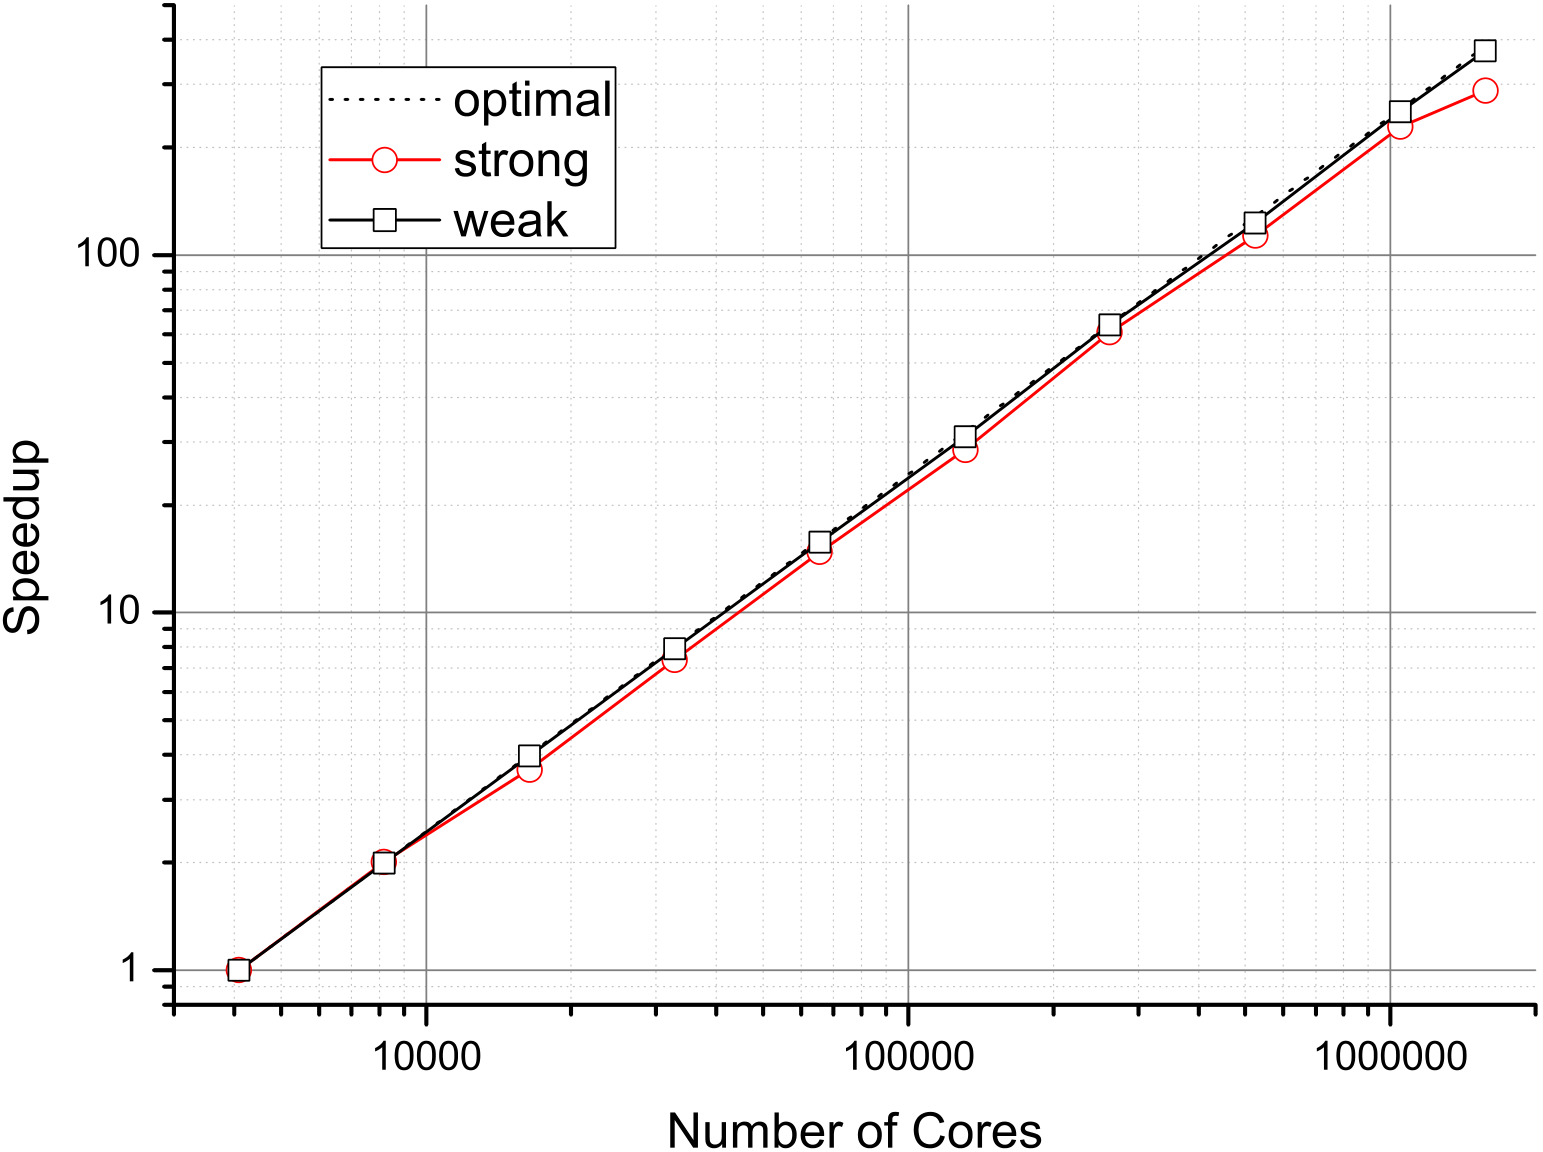
\includegraphics[width=\textwidth]{osiris-scaling}
  \caption{The scaling behaviour of Osiris at the Sequoia system at Lawrence Livermore Labratory.
  Figure 5 reproduced from \textcite{fonseca_exploitingmultiscale_2013}.}%
  \label{fig:osiris-scaling}%
\end{figure}

\begin{table}
  \begin{tabular}{l l l l}
  \toprule
  \textbf{Name} & \textbf{Type} & \textbf{GPU ready} & \textbf{Scalability}\\
  \midrule
  EPOCH & EM 3D & No & MPI\\
  Osiris & EM 3D, RZ*, RZ** & Yes & MPI, OpenMP, SIMD\\
  WarpX & EM 3D, PS*, RZ*, RZ** & Yes & MPI, OpenMP, SIMD\\
  Warp & EM 3D, PS*, RZ*, RZ** & No & MPI, OpenMP\\
  PIConGPU & EM 3D & Yes & MPI, CUDA-ALPAKA\\
  VSim & EM 3D & No & MPI\\
  FBPIC & EM 3D, RZ*** & Yes & MPI, NUMBA\\
  VPIC & EM 3D & No & MPI, pthreads, SIMD\\
  Architect & EM RZ & No & MPI\\
  Wake & QS RZ & No & MPI\\
  QuickPIc & QS RZ & No & MPI\\
  PICLS & EM 3D & No & MPI\\
  \bottomrule
  \end{tabular}
  \caption{Commonly used simulation programs}%
  \label{tab:pic-software}
\end{table}

In the above table we used the following abbreviations
\begin{itemize}
    \item EM: Electromagnetic PIC
    \item QS: Quasi-Static PIC
    \item 3D: Cartesian coordinates, up to 3D
    \item RZ: Cylindrical geometry with FDTD method in \(r\) and \(z\) directions
    \item RZ*: Cylindrical geometry with Fourier azimuthal decomposition
    \item RZ**: Cylindrical geometry with FDTD method in \(r\) direction
                and FFT-based pseudo-spectral method in \(z\) direction
    \item RZ***: Cylindrical geometry with Henkel transform in \(r\) direction
                and FFT-based pseudo-spectral method in \(z\) direction
    \item PS: Pseudo-spectral Maxwell solver with global Fourier transform
    \item PS*: Pseudo-spectral Maxwell solver with domain decomposition and local Fourier transform
\end{itemize}

% tabel ✓(not quite)
% grafic scalabilitate osiris ✓
% mentiune osiris/grup lisabona in ELI whitebook ✓
% coduri de tip WARP de la Bella, citare JL Vay & H Vincenti, picsar ref Vincenti
% referinta tdr eli-np negoita

\section{EPOCH}

\end{document}
